% Generated by Sphinx.
\def\sphinxdocclass{report}
\documentclass[letterpaper,10pt,english]{sphinxmanual}
\usepackage[utf8]{inputenc}
\DeclareUnicodeCharacter{00A0}{\nobreakspace}
\usepackage[T1]{fontenc}
\usepackage{babel}
\usepackage{times}
\usepackage[Bjarne]{fncychap}
\usepackage{longtable}
\usepackage{sphinx}
\usepackage{multirow}


\title{diaGrabber Documentation}
\date{March 04, 2013}
\release{0.1.1}
\author{Karl Bedrich}
\newcommand{\sphinxlogo}{}
\renewcommand{\releasename}{Release}
\makeindex

\makeatletter
\def\PYG@reset{\let\PYG@it=\relax \let\PYG@bf=\relax%
    \let\PYG@ul=\relax \let\PYG@tc=\relax%
    \let\PYG@bc=\relax \let\PYG@ff=\relax}
\def\PYG@tok#1{\csname PYG@tok@#1\endcsname}
\def\PYG@toks#1+{\ifx\relax#1\empty\else%
    \PYG@tok{#1}\expandafter\PYG@toks\fi}
\def\PYG@do#1{\PYG@bc{\PYG@tc{\PYG@ul{%
    \PYG@it{\PYG@bf{\PYG@ff{#1}}}}}}}
\def\PYG#1#2{\PYG@reset\PYG@toks#1+\relax+\PYG@do{#2}}

\expandafter\def\csname PYG@tok@gd\endcsname{\def\PYG@tc##1{\textcolor[rgb]{0.63,0.00,0.00}{##1}}}
\expandafter\def\csname PYG@tok@gu\endcsname{\let\PYG@bf=\textbf\def\PYG@tc##1{\textcolor[rgb]{0.50,0.00,0.50}{##1}}}
\expandafter\def\csname PYG@tok@gt\endcsname{\def\PYG@tc##1{\textcolor[rgb]{0.00,0.27,0.87}{##1}}}
\expandafter\def\csname PYG@tok@gs\endcsname{\let\PYG@bf=\textbf}
\expandafter\def\csname PYG@tok@gr\endcsname{\def\PYG@tc##1{\textcolor[rgb]{1.00,0.00,0.00}{##1}}}
\expandafter\def\csname PYG@tok@cm\endcsname{\let\PYG@it=\textit\def\PYG@tc##1{\textcolor[rgb]{0.25,0.50,0.56}{##1}}}
\expandafter\def\csname PYG@tok@vg\endcsname{\def\PYG@tc##1{\textcolor[rgb]{0.73,0.38,0.84}{##1}}}
\expandafter\def\csname PYG@tok@m\endcsname{\def\PYG@tc##1{\textcolor[rgb]{0.13,0.50,0.31}{##1}}}
\expandafter\def\csname PYG@tok@mh\endcsname{\def\PYG@tc##1{\textcolor[rgb]{0.13,0.50,0.31}{##1}}}
\expandafter\def\csname PYG@tok@cs\endcsname{\def\PYG@tc##1{\textcolor[rgb]{0.25,0.50,0.56}{##1}}\def\PYG@bc##1{\setlength{\fboxsep}{0pt}\colorbox[rgb]{1.00,0.94,0.94}{\strut ##1}}}
\expandafter\def\csname PYG@tok@ge\endcsname{\let\PYG@it=\textit}
\expandafter\def\csname PYG@tok@vc\endcsname{\def\PYG@tc##1{\textcolor[rgb]{0.73,0.38,0.84}{##1}}}
\expandafter\def\csname PYG@tok@il\endcsname{\def\PYG@tc##1{\textcolor[rgb]{0.13,0.50,0.31}{##1}}}
\expandafter\def\csname PYG@tok@go\endcsname{\def\PYG@tc##1{\textcolor[rgb]{0.20,0.20,0.20}{##1}}}
\expandafter\def\csname PYG@tok@cp\endcsname{\def\PYG@tc##1{\textcolor[rgb]{0.00,0.44,0.13}{##1}}}
\expandafter\def\csname PYG@tok@gi\endcsname{\def\PYG@tc##1{\textcolor[rgb]{0.00,0.63,0.00}{##1}}}
\expandafter\def\csname PYG@tok@gh\endcsname{\let\PYG@bf=\textbf\def\PYG@tc##1{\textcolor[rgb]{0.00,0.00,0.50}{##1}}}
\expandafter\def\csname PYG@tok@ni\endcsname{\let\PYG@bf=\textbf\def\PYG@tc##1{\textcolor[rgb]{0.84,0.33,0.22}{##1}}}
\expandafter\def\csname PYG@tok@nl\endcsname{\let\PYG@bf=\textbf\def\PYG@tc##1{\textcolor[rgb]{0.00,0.13,0.44}{##1}}}
\expandafter\def\csname PYG@tok@nn\endcsname{\let\PYG@bf=\textbf\def\PYG@tc##1{\textcolor[rgb]{0.05,0.52,0.71}{##1}}}
\expandafter\def\csname PYG@tok@no\endcsname{\def\PYG@tc##1{\textcolor[rgb]{0.38,0.68,0.84}{##1}}}
\expandafter\def\csname PYG@tok@na\endcsname{\def\PYG@tc##1{\textcolor[rgb]{0.25,0.44,0.63}{##1}}}
\expandafter\def\csname PYG@tok@nb\endcsname{\def\PYG@tc##1{\textcolor[rgb]{0.00,0.44,0.13}{##1}}}
\expandafter\def\csname PYG@tok@nc\endcsname{\let\PYG@bf=\textbf\def\PYG@tc##1{\textcolor[rgb]{0.05,0.52,0.71}{##1}}}
\expandafter\def\csname PYG@tok@nd\endcsname{\let\PYG@bf=\textbf\def\PYG@tc##1{\textcolor[rgb]{0.33,0.33,0.33}{##1}}}
\expandafter\def\csname PYG@tok@ne\endcsname{\def\PYG@tc##1{\textcolor[rgb]{0.00,0.44,0.13}{##1}}}
\expandafter\def\csname PYG@tok@nf\endcsname{\def\PYG@tc##1{\textcolor[rgb]{0.02,0.16,0.49}{##1}}}
\expandafter\def\csname PYG@tok@si\endcsname{\let\PYG@it=\textit\def\PYG@tc##1{\textcolor[rgb]{0.44,0.63,0.82}{##1}}}
\expandafter\def\csname PYG@tok@s2\endcsname{\def\PYG@tc##1{\textcolor[rgb]{0.25,0.44,0.63}{##1}}}
\expandafter\def\csname PYG@tok@vi\endcsname{\def\PYG@tc##1{\textcolor[rgb]{0.73,0.38,0.84}{##1}}}
\expandafter\def\csname PYG@tok@nt\endcsname{\let\PYG@bf=\textbf\def\PYG@tc##1{\textcolor[rgb]{0.02,0.16,0.45}{##1}}}
\expandafter\def\csname PYG@tok@nv\endcsname{\def\PYG@tc##1{\textcolor[rgb]{0.73,0.38,0.84}{##1}}}
\expandafter\def\csname PYG@tok@s1\endcsname{\def\PYG@tc##1{\textcolor[rgb]{0.25,0.44,0.63}{##1}}}
\expandafter\def\csname PYG@tok@gp\endcsname{\let\PYG@bf=\textbf\def\PYG@tc##1{\textcolor[rgb]{0.78,0.36,0.04}{##1}}}
\expandafter\def\csname PYG@tok@sh\endcsname{\def\PYG@tc##1{\textcolor[rgb]{0.25,0.44,0.63}{##1}}}
\expandafter\def\csname PYG@tok@ow\endcsname{\let\PYG@bf=\textbf\def\PYG@tc##1{\textcolor[rgb]{0.00,0.44,0.13}{##1}}}
\expandafter\def\csname PYG@tok@sx\endcsname{\def\PYG@tc##1{\textcolor[rgb]{0.78,0.36,0.04}{##1}}}
\expandafter\def\csname PYG@tok@bp\endcsname{\def\PYG@tc##1{\textcolor[rgb]{0.00,0.44,0.13}{##1}}}
\expandafter\def\csname PYG@tok@c1\endcsname{\let\PYG@it=\textit\def\PYG@tc##1{\textcolor[rgb]{0.25,0.50,0.56}{##1}}}
\expandafter\def\csname PYG@tok@kc\endcsname{\let\PYG@bf=\textbf\def\PYG@tc##1{\textcolor[rgb]{0.00,0.44,0.13}{##1}}}
\expandafter\def\csname PYG@tok@c\endcsname{\let\PYG@it=\textit\def\PYG@tc##1{\textcolor[rgb]{0.25,0.50,0.56}{##1}}}
\expandafter\def\csname PYG@tok@mf\endcsname{\def\PYG@tc##1{\textcolor[rgb]{0.13,0.50,0.31}{##1}}}
\expandafter\def\csname PYG@tok@err\endcsname{\def\PYG@bc##1{\setlength{\fboxsep}{0pt}\fcolorbox[rgb]{1.00,0.00,0.00}{1,1,1}{\strut ##1}}}
\expandafter\def\csname PYG@tok@kd\endcsname{\let\PYG@bf=\textbf\def\PYG@tc##1{\textcolor[rgb]{0.00,0.44,0.13}{##1}}}
\expandafter\def\csname PYG@tok@ss\endcsname{\def\PYG@tc##1{\textcolor[rgb]{0.32,0.47,0.09}{##1}}}
\expandafter\def\csname PYG@tok@sr\endcsname{\def\PYG@tc##1{\textcolor[rgb]{0.14,0.33,0.53}{##1}}}
\expandafter\def\csname PYG@tok@mo\endcsname{\def\PYG@tc##1{\textcolor[rgb]{0.13,0.50,0.31}{##1}}}
\expandafter\def\csname PYG@tok@mi\endcsname{\def\PYG@tc##1{\textcolor[rgb]{0.13,0.50,0.31}{##1}}}
\expandafter\def\csname PYG@tok@kn\endcsname{\let\PYG@bf=\textbf\def\PYG@tc##1{\textcolor[rgb]{0.00,0.44,0.13}{##1}}}
\expandafter\def\csname PYG@tok@o\endcsname{\def\PYG@tc##1{\textcolor[rgb]{0.40,0.40,0.40}{##1}}}
\expandafter\def\csname PYG@tok@kr\endcsname{\let\PYG@bf=\textbf\def\PYG@tc##1{\textcolor[rgb]{0.00,0.44,0.13}{##1}}}
\expandafter\def\csname PYG@tok@s\endcsname{\def\PYG@tc##1{\textcolor[rgb]{0.25,0.44,0.63}{##1}}}
\expandafter\def\csname PYG@tok@kp\endcsname{\def\PYG@tc##1{\textcolor[rgb]{0.00,0.44,0.13}{##1}}}
\expandafter\def\csname PYG@tok@w\endcsname{\def\PYG@tc##1{\textcolor[rgb]{0.73,0.73,0.73}{##1}}}
\expandafter\def\csname PYG@tok@kt\endcsname{\def\PYG@tc##1{\textcolor[rgb]{0.56,0.13,0.00}{##1}}}
\expandafter\def\csname PYG@tok@sc\endcsname{\def\PYG@tc##1{\textcolor[rgb]{0.25,0.44,0.63}{##1}}}
\expandafter\def\csname PYG@tok@sb\endcsname{\def\PYG@tc##1{\textcolor[rgb]{0.25,0.44,0.63}{##1}}}
\expandafter\def\csname PYG@tok@k\endcsname{\let\PYG@bf=\textbf\def\PYG@tc##1{\textcolor[rgb]{0.00,0.44,0.13}{##1}}}
\expandafter\def\csname PYG@tok@se\endcsname{\let\PYG@bf=\textbf\def\PYG@tc##1{\textcolor[rgb]{0.25,0.44,0.63}{##1}}}
\expandafter\def\csname PYG@tok@sd\endcsname{\let\PYG@it=\textit\def\PYG@tc##1{\textcolor[rgb]{0.25,0.44,0.63}{##1}}}

\def\PYGZbs{\char`\\}
\def\PYGZus{\char`\_}
\def\PYGZob{\char`\{}
\def\PYGZcb{\char`\}}
\def\PYGZca{\char`\^}
\def\PYGZam{\char`\&}
\def\PYGZlt{\char`\<}
\def\PYGZgt{\char`\>}
\def\PYGZsh{\char`\#}
\def\PYGZpc{\char`\%}
\def\PYGZdl{\char`\$}
\def\PYGZhy{\char`\-}
\def\PYGZsq{\char`\'}
\def\PYGZdq{\char`\"}
\def\PYGZti{\char`\~}
% for compatibility with earlier versions
\def\PYGZat{@}
\def\PYGZlb{[}
\def\PYGZrb{]}
\makeatother

\begin{document}

\maketitle
\tableofcontents
\phantomsection\label{index::doc}


Contents:


\chapter{Getting started}
\label{getting_started:welcome-to-diagrabber-s-documentation}\label{getting_started:getting-started}\label{getting_started::doc}\label{getting_started:id1}

\section{Installing your doc directory}
\label{getting_started:installing-your-doc-directory}\label{getting_started:installing-docdir}
You may already have sphinx \href{http://sphinx.pocoo.org/}{sphinx}
installed -- you can check by doing:

\begin{Verbatim}[commandchars=\\\{\}]
python -c 'import sphinx'
\end{Verbatim}

If that fails grab the latest version of and install it with:

\begin{Verbatim}[commandchars=\\\{\}]
\textgreater{} sudo easy\_install -U Sphinx
\end{Verbatim}

Now you are ready to build a template for your docs, using
sphinx-quickstart:

\begin{Verbatim}[commandchars=\\\{\}]
\textgreater{} sphinx-quickstart
\end{Verbatim}

accepting most of the defaults.  I choose ``sampledoc'' as the name of my
project.  cd into your new directory and check the contents:

\begin{Verbatim}[commandchars=\\\{\}]
home:\textasciitilde{}/tmp/sampledoc\textgreater{} ls
Makefile      \_static         conf.py
\_build                \_templates      index.rst
\end{Verbatim}

The index.rst is the master ReST for your project, but before adding
anything, let's see if we can build some html:

\begin{Verbatim}[commandchars=\\\{\}]
make html
\end{Verbatim}

If you now point your browser to \code{\_build/html/index.html}, you
should see a basic sphinx site.

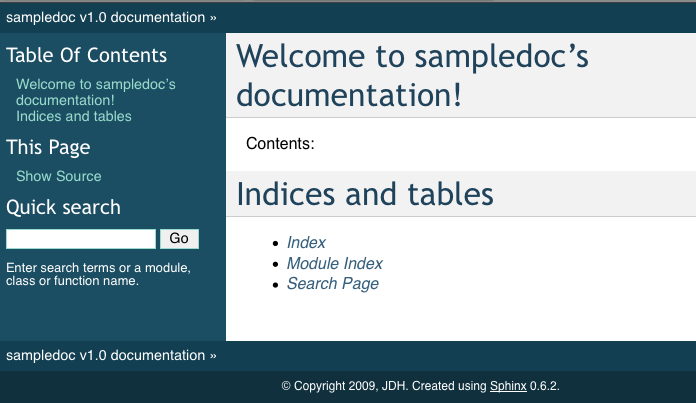
\includegraphics{basic_screenshot.png}


\subsection{Fetching the data}
\label{getting_started:id2}\label{getting_started:fetching-the-data}
Now we will start to customize out docs.  Grab a couple of files from
the \href{http://matplotlib.svn.sourceforge.net/viewvc/matplotlib/trunk/sampledoc\_tut/}{web site}
or svn.  You will need \code{getting\_started.rst} and
\code{\_static/basic\_screenshot.png}.  All of the files live in the
``completed'' version of this tutorial, but since this is a tutorial,
we'll just grab them one at a time, so you can learn what needs to be
changed where.  Since we have more files to come, I'm going to grab
the whole svn directory and just copy the files I need over for now.
First, I'll cd up back into the directory containing my project, check
out the ``finished'' product from svn, and then copy in just the files I
need into my \code{sampledoc} directory:

\begin{Verbatim}[commandchars=\\\{\}]
home:\textasciitilde{}/tmp/sampledoc\textgreater{} pwd
/Users/jdhunter/tmp/sampledoc
home:\textasciitilde{}/tmp/sampledoc\textgreater{} cd ..
home:\textasciitilde{}/tmp\textgreater{} svn co https://matplotlib.svn.sourceforge.net/svnroot/\PYGZbs{}
matplotlib/trunk/sampledoc\_tut
A    sampledoc\_tut/cheatsheet.rst
A    sampledoc\_tut/\_static
A    sampledoc\_tut/\_static/basic\_screenshot.png
A    sampledoc\_tut/conf.py
A    sampledoc\_tut/Makefile
A    sampledoc\_tut/\_templates
A    sampledoc\_tut/\_build
A    sampledoc\_tut/getting\_started.rst
A    sampledoc\_tut/index.rst
Checked out revision 7449.
home:\textasciitilde{}/tmp\textgreater{} cp sampledoc\_tut/getting\_started.rst sampledoc/
home:\textasciitilde{}/tmp\textgreater{} cp sampledoc\_tut/\_static/basic\_screenshot.png \PYGZbs{}
sampledoc/\_static/
\end{Verbatim}

The last step is to modify \code{index.rst} to include the
\code{getting\_started.rst} file (be careful with the indentation, the
``g'' in ``getting\_started'' should line up with the `:' in \code{:maxdepth}:

\begin{Verbatim}[commandchars=\\\{\}]
Contents:

.. toctree::
   :maxdepth: 2

   getting\_started.rst
\end{Verbatim}

and then rebuild the docs:

\begin{Verbatim}[commandchars=\\\{\}]
cd sampledoc
make html
\end{Verbatim}

When you reload the page by refreshing your browser pointing to
\code{\_build/html/index.html}, you should see a link to the
``Getting Started'' docs, and in there this page with the screenshot.
\emph{Voila!}

Note we used the image directive to include to the screenshot above
with:

\begin{Verbatim}[commandchars=\\\{\}]
.. image:: \_static/basic\_screenshot.png
\end{Verbatim}

Next we'll customize the look and feel of our site to give it a logo,
some custom css, and update the navigation panels to look more like
the \href{http://sphinx.pocoo.org/}{sphinx} site itself -- see
\emph{custom\_look}.


\chapter{Defining the source}
\label{source::doc}\label{source:defining-the-source}

\section{plainText}
\label{source:plaintext}\label{source:module-diaGrabber.source.plainText}\index{diaGrabber.source.plainText (module)}\index{plainText (class in diaGrabber.source.plainText)}

\begin{fulllineitems}
\phantomsection\label{source:diaGrabber.source.plainText.plainText}\pysiglinewithargsret{\strong{class }\code{diaGrabber.source.plainText.}\bfcode{plainText}}{\emph{folder}, \emph{file\_name}, \emph{dim\_seperator}, \emph{data\_type='unknown'}}{}
Bases: \code{diaGrabber.source.\_source.\_source}
\index{plainText.dimension (class in diaGrabber.source.plainText)}

\begin{fulllineitems}
\phantomsection\label{source:diaGrabber.source.plainText.plainText.dimension}\pysiglinewithargsret{\strong{class }\bfcode{dimension}}{\emph{name}, \emph{index}}{}
Bases: {\hyperref[dimensions:diaGrabber.source._dimension._dimension]{\code{diaGrabber.source.\_dimension.\_dimension}}}

...test

\end{fulllineitems}


\end{fulllineitems}



\section{stream}
\label{source:module-diaGrabber.source.stream}\label{source:stream}\index{diaGrabber.source.stream (module)}\index{stream (class in diaGrabber.source.stream)}

\begin{fulllineitems}
\phantomsection\label{source:diaGrabber.source.stream.stream}\pysiglinewithargsret{\strong{class }\code{diaGrabber.source.stream.}\bfcode{stream}}{\emph{command}, \emph{start\_via}, \emph{stop\_via}, \emph{dim\_seperator}, \emph{data\_type='unknown'}, \emph{key\_to\_end\_process='`}, \emph{readoutEverNLine=1}, \emph{infoEveryNLines=1000}}{}~\index{stream.dimension (class in diaGrabber.source.stream)}

\begin{fulllineitems}
\phantomsection\label{source:diaGrabber.source.stream.stream.dimension}\pysiglinewithargsret{\strong{class }\bfcode{dimension}}{\emph{name}, \emph{index}}{}
...test

\end{fulllineitems}

\index{getInfoEveryNLines() (diaGrabber.source.stream.stream method)}

\begin{fulllineitems}
\phantomsection\label{source:diaGrabber.source.stream.stream.getInfoEveryNLines}\pysiglinewithargsret{\code{stream.}\bfcode{getInfoEveryNLines}}{}{}
\end{fulllineitems}

\index{getReadoutEverNLine() (diaGrabber.source.stream.stream method)}

\begin{fulllineitems}
\phantomsection\label{source:diaGrabber.source.stream.stream.getReadoutEverNLine}\pysiglinewithargsret{\code{stream.}\bfcode{getReadoutEverNLine}}{}{}
\end{fulllineitems}

\index{setInfoEveryNLines() (diaGrabber.source.stream.stream method)}

\begin{fulllineitems}
\phantomsection\label{source:diaGrabber.source.stream.stream.setInfoEveryNLines}\pysiglinewithargsret{\code{stream.}\bfcode{setInfoEveryNLines}}{\emph{nLines}}{}
\end{fulllineitems}

\index{setReadoutEverNLine() (diaGrabber.source.stream.stream method)}

\begin{fulllineitems}
\phantomsection\label{source:diaGrabber.source.stream.stream.setReadoutEverNLine}\pysiglinewithargsret{\code{stream.}\bfcode{setReadoutEverNLine}}{\emph{nLine}}{}
\end{fulllineitems}


\end{fulllineitems}



\section{plainTextStream}
\label{source:module-diaGrabber.source.plainTextStream}\label{source:plaintextstream}\index{diaGrabber.source.plainTextStream (module)}\index{plainTextStream (class in diaGrabber.source.plainTextStream)}

\begin{fulllineitems}
\phantomsection\label{source:diaGrabber.source.plainTextStream.plainTextStream}\pysiglinewithargsret{\strong{class }\code{diaGrabber.source.plainTextStream.}\bfcode{plainTextStream}}{\emph{command}, \emph{start\_via}, \emph{stop\_via}, \emph{dim\_seperator}, \emph{output\_file}, \emph{data\_type='unknown'}, \emph{key\_to\_end\_process='`}, \emph{readoutEverNLine=1}, \emph{infoEveryNLines=1000}}{}
Bases: \code{diaGrabber.source.\_source.\_source}
\index{plainTextStream.dimension (class in diaGrabber.source.plainTextStream)}

\begin{fulllineitems}
\phantomsection\label{source:diaGrabber.source.plainTextStream.plainTextStream.dimension}\pysiglinewithargsret{\strong{class }\bfcode{dimension}}{\emph{name}, \emph{index}}{}
Bases: {\hyperref[dimensions:diaGrabber.source._dimension._dimension]{\code{diaGrabber.source.\_dimension.\_dimension}}}

...test

\end{fulllineitems}

\index{getInfoEveryNLines() (diaGrabber.source.plainTextStream.plainTextStream method)}

\begin{fulllineitems}
\phantomsection\label{source:diaGrabber.source.plainTextStream.plainTextStream.getInfoEveryNLines}\pysiglinewithargsret{\code{plainTextStream.}\bfcode{getInfoEveryNLines}}{}{}
\end{fulllineitems}

\index{getReadoutEverNLine() (diaGrabber.source.plainTextStream.plainTextStream method)}

\begin{fulllineitems}
\phantomsection\label{source:diaGrabber.source.plainTextStream.plainTextStream.getReadoutEverNLine}\pysiglinewithargsret{\code{plainTextStream.}\bfcode{getReadoutEverNLine}}{}{}
\end{fulllineitems}

\index{setInfoEveryNLines() (diaGrabber.source.plainTextStream.plainTextStream method)}

\begin{fulllineitems}
\phantomsection\label{source:diaGrabber.source.plainTextStream.plainTextStream.setInfoEveryNLines}\pysiglinewithargsret{\code{plainTextStream.}\bfcode{setInfoEveryNLines}}{\emph{nLines}}{}
\end{fulllineitems}

\index{setReadoutEverNLine() (diaGrabber.source.plainTextStream.plainTextStream method)}

\begin{fulllineitems}
\phantomsection\label{source:diaGrabber.source.plainTextStream.plainTextStream.setReadoutEverNLine}\pysiglinewithargsret{\code{plainTextStream.}\bfcode{setReadoutEverNLine}}{\emph{nLine}}{}
\end{fulllineitems}


\end{fulllineitems}



\chapter{Attach dimensions}
\label{dimensions::doc}\label{dimensions:attach-dimensions}\index{\_dimension (class in diaGrabber.source.\_dimension)}

\begin{fulllineitems}
\phantomsection\label{dimensions:diaGrabber.source._dimension._dimension}\pysiglinewithargsret{\strong{class }\code{diaGrabber.source.\_dimension.}\bfcode{\_dimension}}{\emph{name}, \emph{index}}{}~\index{includeAll() (diaGrabber.source.\_dimension.\_dimension method)}

\begin{fulllineitems}
\phantomsection\label{dimensions:diaGrabber.source._dimension._dimension.includeAll}\pysiglinewithargsret{\bfcode{includeAll}}{\emph{resolution}}{}
Include all values and sort in a range from min to max values
dissolved by the resolution
!!!: not all sources can define the min and max values

\end{fulllineitems}

\index{includeChronic() (diaGrabber.source.\_dimension.\_dimension method)}

\begin{fulllineitems}
\phantomsection\label{dimensions:diaGrabber.source._dimension._dimension.includeChronic}\pysiglinewithargsret{\bfcode{includeChronic}}{\emph{resolution}}{}
Only take the last {[}dimension.resolution{]} values
override when read more than that

\end{fulllineitems}

\index{includeFromTo() (diaGrabber.source.\_dimension.\_dimension method)}

\begin{fulllineitems}
\phantomsection\label{dimensions:diaGrabber.source._dimension._dimension.includeFromTo}\pysiglinewithargsret{\bfcode{includeFromTo}}{\emph{from\_value}, \emph{to\_value}, \emph{resolution}}{}
\end{fulllineitems}

\index{setCalcToValue() (diaGrabber.source.\_dimension.\_dimension method)}

\begin{fulllineitems}
\phantomsection\label{dimensions:diaGrabber.source._dimension._dimension.setCalcToValue}\pysiglinewithargsret{\bfcode{setCalcToValue}}{\emph{calc\_index}}{}
set every value of the dimension to the result of one
entry in dimension.calc

\end{fulllineitems}

\index{setCounter() (diaGrabber.source.\_dimension.\_dimension method)}

\begin{fulllineitems}
\phantomsection\label{dimensions:diaGrabber.source._dimension._dimension.setCounter}\pysiglinewithargsret{\bfcode{setCounter}}{\emph{start=0}, \emph{delta=1}}{}
\end{fulllineitems}

\index{setPlotOnlyRecentPosition() (diaGrabber.source.\_dimension.\_dimension method)}

\begin{fulllineitems}
\phantomsection\label{dimensions:diaGrabber.source._dimension._dimension.setPlotOnlyRecentPosition}\pysiglinewithargsret{\bfcode{setPlotOnlyRecentPosition}}{}{}
\end{fulllineitems}

\index{setPlotRange() (diaGrabber.source.\_dimension.\_dimension method)}

\begin{fulllineitems}
\phantomsection\label{dimensions:diaGrabber.source._dimension._dimension.setPlotRange}\pysiglinewithargsret{\bfcode{setPlotRange}}{\emph{start}, \emph{stop}, \emph{step}}{}
type `None' if you don't want to define the input

\end{fulllineitems}


\end{fulllineitems}



\section{Installing your doc directory}
\label{dimensions:installing-your-doc-directory}
Dimension von source entkoppeln
methods in dim rein


\chapter{Methods to ...}
\label{methods:methods-to}\label{methods::doc}\label{methods:module-diaGrabber.methods.calc}\index{diaGrabber.methods.calc (module)}
Includes all classes for calculations for off-the-reel-taken-values of a source-class
\index{delta (class in diaGrabber.methods.calc)}

\begin{fulllineitems}
\phantomsection\label{methods:diaGrabber.methods.calc.delta}\pysiglinewithargsret{\strong{class }\code{diaGrabber.methods.calc.}\bfcode{delta}}{\emph{n}}{}
calc. the mean-difference of the last n values

\end{fulllineitems}

\index{divideCalcClasses (class in diaGrabber.methods.calc)}

\begin{fulllineitems}
\phantomsection\label{methods:diaGrabber.methods.calc.divideCalcClasses}\pysiglinewithargsret{\strong{class }\code{diaGrabber.methods.calc.}\bfcode{divideCalcClasses}}{\emph{upperCalcClass}, \emph{lowerCalcClass}}{}
divide the last calulated values of two given calc-classes
use it like this:
dim1 = myFile.dimension(...)
dim1.calc.append(calc.delta(10))

dim2 = myFile.dimension(...)
dim2.calc.append(calc.delta(10))
\#\textless{}\textless{}\textless{}
dim2.calc.append(dim1.calc{[}0{]}, dim2.calc{[}0{]})
\#\textgreater{}\textgreater{}\textgreater{}
\#In this case the derivate d(dim1)/d(dim2) middled for the last 10
\#valued will be calculated
This procedure will only work if both dimensions are in merge or basis.

\end{fulllineitems}

\index{mean (class in diaGrabber.methods.calc)}

\begin{fulllineitems}
\phantomsection\label{methods:diaGrabber.methods.calc.mean}\pysiglinewithargsret{\strong{class }\code{diaGrabber.methods.calc.}\bfcode{mean}}{\emph{n}}{}
calc. the mean of the last n values

\end{fulllineitems}

\phantomsection\label{methods:module-diaGrabber.methods.merge}\index{diaGrabber.methods.merge (module)}\index{max (class in diaGrabber.methods.merge)}

\begin{fulllineitems}
\phantomsection\label{methods:diaGrabber.methods.merge.max}\pysigline{\strong{class }\code{diaGrabber.methods.merge.}\bfcode{max}}
\end{fulllineitems}

\index{mean (class in diaGrabber.methods.merge)}

\begin{fulllineitems}
\phantomsection\label{methods:diaGrabber.methods.merge.mean}\pysigline{\strong{class }\code{diaGrabber.methods.merge.}\bfcode{mean}}
\end{fulllineitems}

\index{min (class in diaGrabber.methods.merge)}

\begin{fulllineitems}
\phantomsection\label{methods:diaGrabber.methods.merge.min}\pysigline{\strong{class }\code{diaGrabber.methods.merge.}\bfcode{min}}
\end{fulllineitems}

\index{sum (class in diaGrabber.methods.merge)}

\begin{fulllineitems}
\phantomsection\label{methods:diaGrabber.methods.merge.sum}\pysigline{\strong{class }\code{diaGrabber.methods.merge.}\bfcode{sum}}
\end{fulllineitems}

\phantomsection\label{methods:module-diaGrabber.methods.exclude}\index{diaGrabber.methods.exclude (module)}
Includes all classes for criteria to exclude
off-the-reel-taken-values of a source-class
private methods \_get will return True if the value fullfills the criteria and
falas if it fails.
\index{calcBiggerValue (class in diaGrabber.methods.exclude)}

\begin{fulllineitems}
\phantomsection\label{methods:diaGrabber.methods.exclude.calcBiggerValue}\pysiglinewithargsret{\strong{class }\code{diaGrabber.methods.exclude.}\bfcode{calcBiggerValue}}{\emph{calcClass}, \emph{value}}{}
exclude value if result of a calc.xx-class
is bigger than the given value

\end{fulllineitems}

\index{calcSmallerCalc (class in diaGrabber.methods.exclude)}

\begin{fulllineitems}
\phantomsection\label{methods:diaGrabber.methods.exclude.calcSmallerCalc}\pysiglinewithargsret{\strong{class }\code{diaGrabber.methods.exclude.}\bfcode{calcSmallerCalc}}{\emph{dim1}, \emph{dim2}}{}
exclude value if result of dimension.calc{[}dim1{]}
is smaller than dimension.calc{[}dim2{]}

\end{fulllineitems}

\index{calcSmallerValue (class in diaGrabber.methods.exclude)}

\begin{fulllineitems}
\phantomsection\label{methods:diaGrabber.methods.exclude.calcSmallerValue}\pysiglinewithargsret{\strong{class }\code{diaGrabber.methods.exclude.}\bfcode{calcSmallerValue}}{\emph{calcClass}, \emph{value}}{}
exclude value if result of a calc.xx-class
is smaller than the given value

\end{fulllineitems}

\phantomsection\label{methods:module-diaGrabber.methods.transform}\index{diaGrabber.methods.transform (module)}\index{fx (class in diaGrabber.methods.transform)}

\begin{fulllineitems}
\phantomsection\label{methods:diaGrabber.methods.transform.fx}\pysiglinewithargsret{\strong{class }\code{diaGrabber.methods.transform.}\bfcode{fx}}{\emph{fx\_str}, \emph{name}}{}~\index{get() (diaGrabber.methods.transform.fx method)}

\begin{fulllineitems}
\phantomsection\label{methods:diaGrabber.methods.transform.fx.get}\pysiglinewithargsret{\bfcode{get}}{\emph{x}}{}
\end{fulllineitems}


\end{fulllineitems}

\index{interpolationTable (class in diaGrabber.methods.transform)}

\begin{fulllineitems}
\phantomsection\label{methods:diaGrabber.methods.transform.interpolationTable}\pysiglinewithargsret{\strong{class }\code{diaGrabber.methods.transform.}\bfcode{interpolationTable}}{\emph{source\_l}, \emph{name}}{}~\index{get() (diaGrabber.methods.transform.interpolationTable method)}

\begin{fulllineitems}
\phantomsection\label{methods:diaGrabber.methods.transform.interpolationTable.get}\pysiglinewithargsret{\bfcode{get}}{\emph{time}}{}
conform to the openFoam-class of the same name
print an linear-interpolated value to a given time{[}float{]}
source\_l = {[} {[}time1,value1{]}, ... , {[}timeN,valueN{]} {]}

\end{fulllineitems}


\end{fulllineitems}



\chapter{Defining the Target}
\label{target::doc}\label{target:target}\label{target:defining-the-target}

\section{Matrix}
\label{target:matrix}\index{coarseMatrix (class in diaGrabber.target)}

\begin{fulllineitems}
\phantomsection\label{target:diaGrabber.target.coarseMatrix}\pysiglinewithargsret{\strong{class }\code{diaGrabber.target.}\bfcode{coarseMatrix}}{\emph{basis\_dim}, \emph{merge\_dim}, \emph{derivate\_dim}, \emph{sourceClass}}{}
Bases: \code{diaGrabber.target.matrix.\_matrix}

\end{fulllineitems}

\index{fineMatrix (class in diaGrabber.target)}

\begin{fulllineitems}
\phantomsection\label{target:diaGrabber.target.fineMatrix}\pysiglinewithargsret{\strong{class }\code{diaGrabber.target.}\bfcode{fineMatrix}}{\emph{basis\_dim}, \emph{merge\_dim}, \emph{derivate\_dim}, \emph{sourceClass}}{}
Bases: \code{diaGrabber.target.matrix.\_matrix}
\begin{quote}

This class isn't as fast as \code{coarseMatrix} but can assign values
in a more accurate way if the following condition is fullfilled:
\end{quote}

\begin{notice}{note}{Note:}
number of datapoints in matrix\textgreater{}\textgreater{} matrix-resolution
\end{notice}

\begin{tabulary}{\linewidth}{|L|L|L|}
\hline

1
 & 
2
 & 
3
\\\hline

4
 & 
5
 & 
6
\\\hline

7
 & 
8
 & 
9
\\\hline
\end{tabulary}


\end{fulllineitems}



\section{discrete Points}
\label{target:discrete-points}\label{target:module-diaGrabber.target.discretePoints}\index{diaGrabber.target.discretePoints (module)}

\chapter{Indices and tables}
\label{index:indices-and-tables}\begin{itemize}
\item {} 
\emph{genindex}

\item {} 
\emph{modindex}

\item {} 
\emph{search}

\end{itemize}


\renewcommand{\indexname}{Python Module Index}
\begin{theindex}
\def\bigletter#1{{\Large\sffamily#1}\nopagebreak\vspace{1mm}}
\bigletter{d}
\item {\texttt{diaGrabber.methods.calc}}, \pageref{methods:module-diaGrabber.methods.calc}
\item {\texttt{diaGrabber.methods.exclude}}, \pageref{methods:module-diaGrabber.methods.exclude}
\item {\texttt{diaGrabber.methods.merge}}, \pageref{methods:module-diaGrabber.methods.merge}
\item {\texttt{diaGrabber.methods.transform}}, \pageref{methods:module-diaGrabber.methods.transform}
\item {\texttt{diaGrabber.source.plainText}}, \pageref{source:module-diaGrabber.source.plainText}
\item {\texttt{diaGrabber.source.plainTextStream}}, \pageref{source:module-diaGrabber.source.plainTextStream}
\item {\texttt{diaGrabber.source.stream}}, \pageref{source:module-diaGrabber.source.stream}
\item {\texttt{diaGrabber.target.discretePoints}}, \pageref{target:module-diaGrabber.target.discretePoints}
\end{theindex}

\renewcommand{\indexname}{Index}
\printindex
\end{document}
